\documentclass[11pt,]{article}
\usepackage[left=1in,top=1in,right=1in,bottom=1in]{geometry}
\newcommand*{\authorfont}{\fontfamily{phv}\selectfont}
\usepackage[]{mathpazo}


  \usepackage[T1]{fontenc}
  \usepackage[utf8]{inputenc}



\usepackage{abstract}
\renewcommand{\abstractname}{}    % clear the title
\renewcommand{\absnamepos}{empty} % originally center

\renewenvironment{abstract}
 {{%
    \setlength{\leftmargin}{0mm}
    \setlength{\rightmargin}{\leftmargin}%
  }%
  \relax}
 {\endlist}

\makeatletter
\def\@maketitle{%
  \newpage
%  \null
%  \vskip 2em%
%  \begin{center}%
  \let \footnote \thanks
    {\fontsize{18}{20}\selectfont\raggedright  \setlength{\parindent}{0pt} \@title \par}%
}
%\fi
\makeatother




\setcounter{secnumdepth}{3}


\usepackage{graphicx,grffile}
\makeatletter
\def\maxwidth{\ifdim\Gin@nat@width>\linewidth\linewidth\else\Gin@nat@width\fi}
\def\maxheight{\ifdim\Gin@nat@height>\textheight\textheight\else\Gin@nat@height\fi}
\makeatother
% Scale images if necessary, so that they will not overflow the page
% margins by default, and it is still possible to overwrite the defaults
% using explicit options in \includegraphics[width, height, ...]{}
\setkeys{Gin}{width=\maxwidth,height=\maxheight,keepaspectratio}

\title{Título\\
Subtítulo\\
Subtítulo  }



\author{\Large Cinthia Amalia Vandepool Candelario\vspace{0.05in} \newline\normalsize\emph{Estudiante de Geografia, Universidad Autónoma de Santo Domingo (UASD)}  }


\date{}

\usepackage{titlesec}

\titleformat*{\section}{\normalsize\bfseries}
\titleformat*{\subsection}{\normalsize\itshape}
\titleformat*{\subsubsection}{\normalsize\itshape}
\titleformat*{\paragraph}{\normalsize\itshape}
\titleformat*{\subparagraph}{\normalsize\itshape}

\titlespacing{\section}
{0pt}{36pt}{0pt}
\titlespacing{\subsection}
{0pt}{36pt}{0pt}
\titlespacing{\subsubsection}
{0pt}{36pt}{0pt}





\newtheorem{hypothesis}{Hypothesis}
\usepackage{setspace}

\makeatletter
\@ifpackageloaded{hyperref}{}{%
\ifxetex
  \PassOptionsToPackage{hyphens}{url}\usepackage[setpagesize=false, % page size defined by xetex
              unicode=false, % unicode breaks when used with xetex
              xetex]{hyperref}
\else
  \PassOptionsToPackage{hyphens}{url}\usepackage[unicode=true]{hyperref}
\fi
}

\@ifpackageloaded{color}{
    \PassOptionsToPackage{usenames,dvipsnames}{color}
}{%
    \usepackage[usenames,dvipsnames]{color}
}
\makeatother
\hypersetup{breaklinks=true,
            bookmarks=true,
            pdfauthor={Cinthia Amalia Vandepool Candelario (Estudiante de Geografia, Universidad Autónoma de Santo Domingo (UASD))},
             pdfkeywords = {morfometría fluvial, modelo digital de elevación, red de drenaje, razón
de bifurcación},  
            pdftitle={Título\\
Subtítulo\\
Subtítulo},
            colorlinks=true,
            citecolor=blue,
            urlcolor=blue,
            linkcolor=magenta,
            pdfborder={0 0 0}}
\urlstyle{same}  % don't use monospace font for urls

% set default figure placement to htbp
\makeatletter
\def\fps@figure{htbp}
\makeatother

\usepackage{pdflscape} \newcommand{\blandscape}{\begin{landscape}}
\newcommand{\elandscape}{\end{landscape}}


% add tightlist ----------
\providecommand{\tightlist}{%
\setlength{\itemsep}{0pt}\setlength{\parskip}{0pt}}

\begin{document}
	
% \pagenumbering{arabic}% resets `page` counter to 1 
%
% \maketitle

{% \usefont{T1}{pnc}{m}{n}
\setlength{\parindent}{0pt}
\thispagestyle{plain}
{\fontsize{18}{20}\selectfont\raggedright 
\maketitle  % title \par  

}

{
   \vskip 13.5pt\relax \normalsize\fontsize{11}{12} 
\textbf{\authorfont Cinthia Amalia Vandepool Candelario} \hskip 15pt \emph{\small Estudiante de Geografia, Universidad Autónoma de Santo Domingo (UASD)}   

}

}








\begin{abstract}

    \hbox{\vrule height .2pt width 39.14pc}

    \vskip 8.5pt % \small 

\noindent Resumen del manuscrito


\vskip 8.5pt \noindent \emph{Keywords}: morfometría fluvial, modelo digital de elevación, red de drenaje, razón
de bifurcación \par

    \hbox{\vrule height .2pt width 39.14pc}



\end{abstract}


\vskip 6.5pt


\noindent  \section{Introducción}\label{introducciuxf3n}

A lo largo del ultimo siglo se ha reducido la dificultad para realizar
analisis espaciales gracias a los novedosos avances tecnologicos, el
desarrollo de los Sistemas de Información Geografica (SIG) ha
simplificado el arduo trabajo que suponia \{llevar acabo analisis
espaciales\}, aunque a pesar de todas las herramientas \{\} disponibles
la República Dominicana aún esta pasos por detras de muchos país en
especial en lo relacionado a los analisis morfometricos de cuencas
hidrograficas, situación lamentable ya que la isla posee innumerables
cursos de agua permitiendole ocupar un lugar privilegiado en este siglo
ya que cada día más país sufren por la escases de agua dulce potable.

La morfometría fluvial se encarga de analizar los parámetros
geomorfológicos de una cuenca hidrográfica, tales como la red de
drenaje, la pendiente, la forma, el orden de la red y demás aspectos
fisicos.(@) Entendiendo que la cuenca hidrográfica es ese sistema o
unidad geográfica e hidrológica formada por un rio principal y todo el
territorio entre el origen del rio y su desembocadura, interactúando en
este espacio diversos factores bióticos y abióticos.

El aspecto general de una cuenca y de su red se entiende como la forma
depende de la gravedad y la pendiente

El orden de red indica el grado de ramificacion de una red fluvial
existen distintos metodos para jerarquizar los cursos de una red, los
dos más conocidos y utilizados son el metodo de Strahler (1952) y el de
Horton (1945), gracias a esta jerarquización se puede tener entender
mejor el comportamiento del sistema de drenaje de la cuenca, ademas de
que se puede obtener la razon de bifurcación descrita por Horton como la
relación entre el número de cursos de un orden y número de cursos de
orden más alto, esta propiedad es condicionada por la forma que presenta
la cuenca (Elorza (2008) Lux Cardona (2016) Ibañez Asensio, Moreno
Ramón, \& Gisbert Blanquer (2011)).

Perfiles longitudinales e índice de concavidad de cursos más largos

La cuenca hidrográfica a analizar en esta investigación es la Subcuenca
Caña perteneciente a la Cuenca del Rio Macasia, ubicada en el extremo
suroeste de la República Dominicana, dicho análisis se realizará
basandonos en datos preexistentes a partir de un \emph{modelo digital de
elevación (DEM)}, el cual es un modelo simbólico, de estructura numérica
y digital que pretende representar la distribución espacial de la
elevación del terreno, siendo la altura una variable escalar que se
distribuye en un espacio bi-dimensional (Burgos \& Salcedo (2014)).

Debido a la escases de datos sobre las caracteristicas morfometricas de
las cuencas de la República Dominicana esta investigación pretende
aportar datos reales sobre la morfometria de la microcuenca caña con el
objetivo de que sean utiles para realizar futuros estudios sobre el
comportamiento hidrologico de la microcuenca ante eventos climaticos y
su posible incidencia en las poblaciones asentadas en su margen; para
dicho objetivo estaremos formulando distintas hipotesis que nos
permitiran entender la dinamica de nuentra región de estudio empleado
para esto distintas herramientas geoespaciales de codigo abierto.

\section{Metodología}\label{metodologuxeda}

\subsection{Área de Estudio}\label{uxe1rea-de-estudio}

Respecto a la division politico-administrativa la cuenca del Rio Caña
abarca los municipios de El Cercado y Las Matas de Farfan en la
provincia de San Juan y las comunidades de El Llano, Juan Santiago y
Hondo Valle de la provinica de Elias Piña. Geograficamente se localiza
entre las coordenadas 18\(^\circ\) 56' 25.32" N y 18\(^\circ\) 37'
39.64" N latitud norte y 71\(^\circ\) 27' 18.45" W y 71\(^\circ\) 44'
03.63" W longitud oeste Ministerio de Medio ambiente y Recursos
naturales (2016). El rio caña nace en la sierra de neiba aproximadamente
a unos 1,155 metros sobre el nievel del mar.

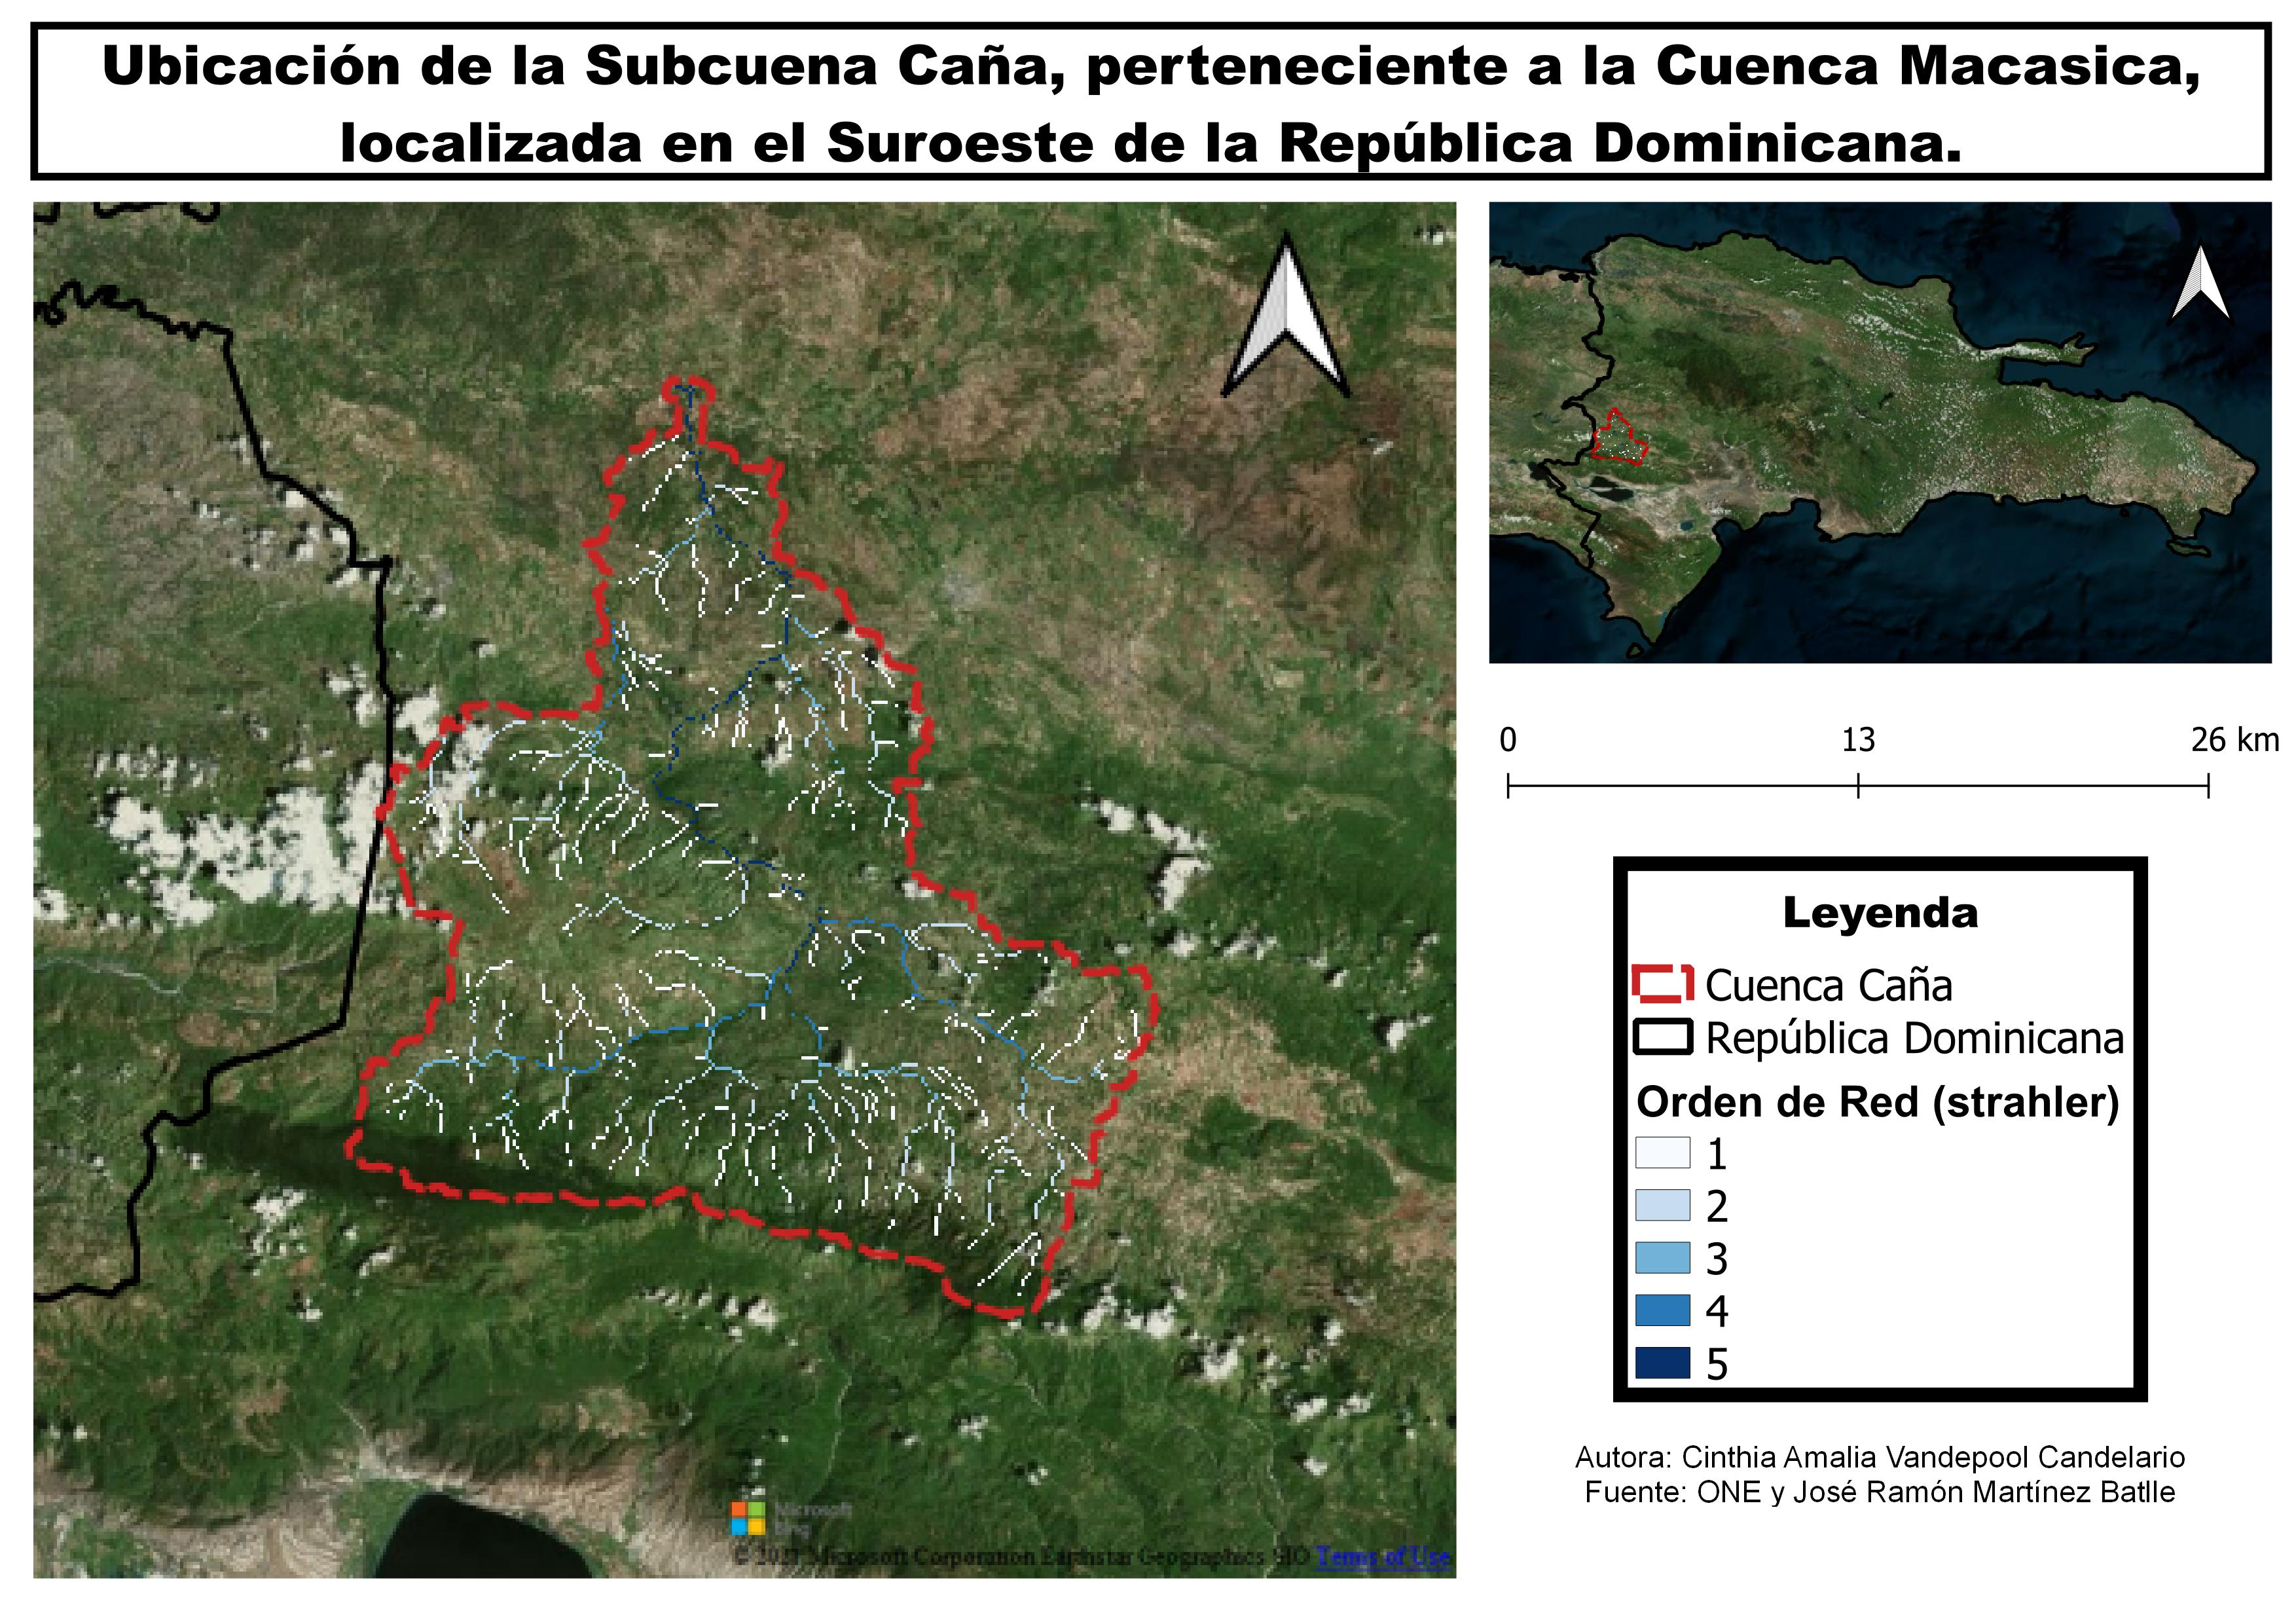
\includegraphics[width=0.75000\textwidth]{mapa_de_subcuenca_cana.jpg} De
acuerdo al mapa Zonas de Vida (OEA, 1967), la mayor superficie de la
cuenca lo ocupa el Bosque humedo subtropical, se caracteriza por
presentar topografía que varía desde plana hasta accidentada con un
patrón de lluvia que varía de 1000 mm. a 2000 mm.. Según la ubicación de
las áreas, la biotemperatura media anual es de 23ºC a 24º C con una
evapotranspiración potencial estimada en promedio como 20\% menor que la
precipitación media total anual. El Bosque muy húmedo Montano Bajo es la
segunda en extensión, se caracteriza por la presencia de escarchas
temporales, precipitaciones que alcanzar cantidades mayores a los 2,000
mm. totales anuales con una evapotranspiración potencial estimada en
promedio en 55\% menor que la precipitación media total anual,
topografía generalmente accidentada con elevaciones que van desde los
850 hasta los 2,100 metros y en menor proporcion lo ocupa el bosque
humedo montano bajo Ministerio de Medio ambiente y Recursos naturales
(2016).

La mayor parte de la cuenca discurre sobre el sistema geomorfologico de
la sierra de neiba y en menor proporción sobre el valle de San juan,
siendo la geología conformada, en mayor proporción, por Caliza tipo
Neiba, Marga con calcarenita tipo sombrerito, Marga con intercalaciones
de bancos de caliza arenosa, arenisca, marga arenosa, conglomerados,
conglomerados poligenico, molasa marina y continental y arena; y en
menor proporción esta conformada por caliza en bancos de espesores
variables con nodulos e intercalaciones de pedernal de color
blanco-crema, depositos fluviales, depositos cuaternarios
indiferenciados, Basaltos, Tobas, Aglormerados y Rocas Volcánicas
Submarinas Ministerio de Medio ambiente y Recursos naturales (2016).

\begin{figure}
\centering
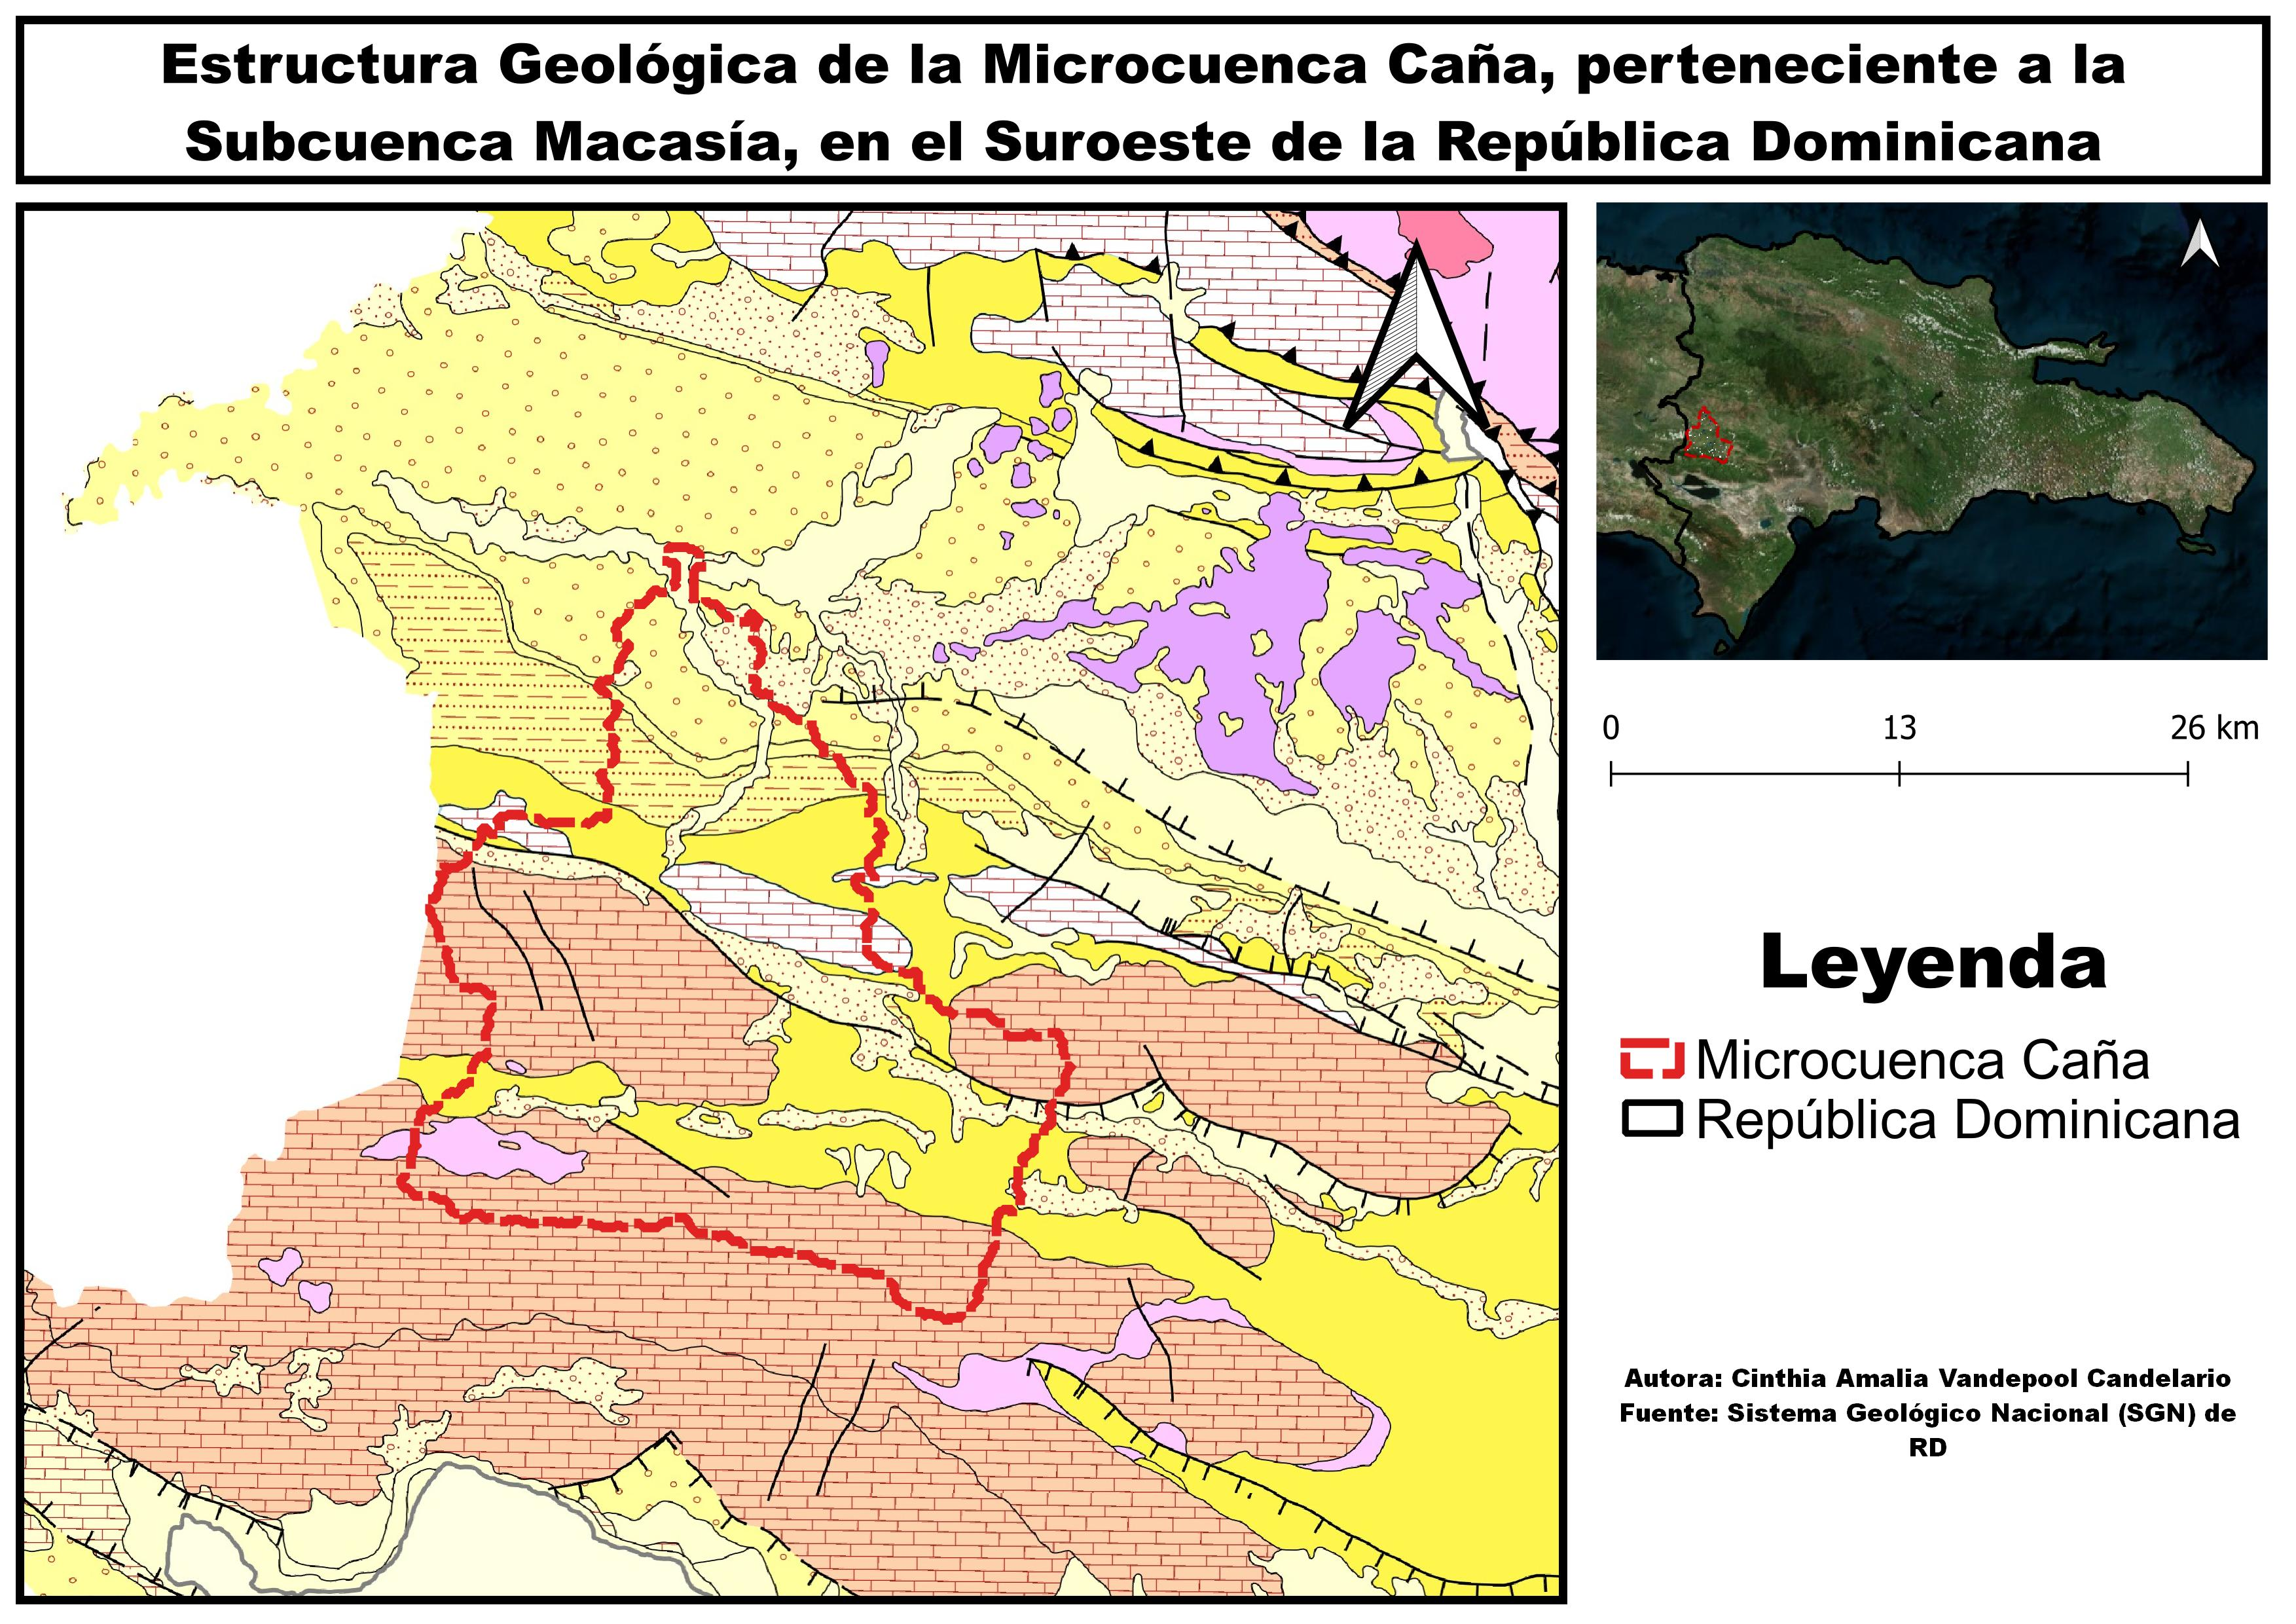
\includegraphics[width=0.75000\textwidth]{mapa_geologico_cuenca_cana.jpg}
\caption{Estructura Geológica de la Cuenca Caña}
\end{figure}

\subsection{Metodología}\label{metodologuxeda-1}

Para la elaboración de esta investigación se emplearon métodos de
analisis morfometrico a partir de un DEM de la cuenca de interes,
inicialmente cargue una serie de paquetes de Grass en R adecuando el
entorno para ejectar los codigos necesarios.

En primer lugar, se importó a R, como SpatialGridDataFrame, un DEM
alojado en la base de datos de GRASS GIS, se estableció su ruta y
conviertiendolo a su vez en un objeto raster por medio del paquete
raster de R; partiendo del complemento \emph{r.watershed} (el cual
generá un conjunto de mapas que indican: \emph{la acumulación de flujo,
la dirección del drenaje, la ubicación de los arroyos y las cuencas
hidrográficas} (GRASS Development Team (2003g))) y del modelo digital de
elevaciones (DEM) se generaron diversas capas calculando así los
parámetros hidrográficos de la cuenca del rio caña y sus redes de
drenaje, además, seguido a esto se importó un conjunto de capas ráster
de GRASS GIS a R, como el mapa de red de drenaje y el mapa de cuencas
visualizandolas por medio de \emph{leaflet}.

Utilizando el complemento de GRASS GIS \emph{r.water.outlet} (GRASS
Development Team (2003f)) y apoyandose en los paquetes \emph{mapview}
(Tim Appelhans and others (2020)) y \emph{leaflet} se extrajó la cuenca
de drenaje a partir de un mapa de dirección de flujos con un umbral de
acumulación de \emph{80 celdas} y las coordenadas de la desembocadura de
la cuenca cana (-71.62524,18.94026).

Posteriormente se estableció una máscara usando el límite de la cuenca
caña para luego realizar la extracción, partir del DEM, de la red de
drenaje utilizando el complemento de GRASS GIS \emph{r.stream.extract}
(GRASS Development Team (2003d)) desde R. Tras esto, se utilizó el
complemento \emph{r.stream}(GRASS Development Team (2003e)) para generar
un mapa de dirección de flujo, \emph{r.stream.order} (GRASS Development
Team (2003b)) para un mapa de orden de red según varios métodos, entre
ellos el método de Strahler y de Horton, a partir de
\emph{r.stream.basins} (GRASS Development Team (2003c)) un mapa de
cuencas según órdenes de red y apoyandose del complemento
\emph{r.stream.stats}(GRASS Development Team (2003a)) se generó las
estadísticas de red resumidas por órdenes, incluyendo la razón de
bifurcación.

\section{Resultados}\label{resultados}

\ldots

\section{Discusión}\label{discusiuxf3n}

\section{Agradecimientos}\label{agradecimientos}

\section{Información de soporte}\label{informaciuxf3n-de-soporte}

\ldots

\section{\texorpdfstring{\emph{Script}
reproducible}{Script reproducible}}\label{script-reproducible}

\ldots

\section*{Referencias}\label{referencias}
\addcontentsline{toc}{section}{Referencias}

\hypertarget{refs}{}
\hypertarget{ref-burgos2014modelos}{}
Burgos, V. H., \& Salcedo, A. P. (2014). Modelos digitales de elevación:
Tendencias, correcciones hidrológicas y nuevas fuentes de información.
\emph{Encuentro de Investigadores En Formación En Recursos Hídricos (2,
2014, Ezeiza, Buenos Aires, Argentina). Disponible En: Http://Www. Ina.
Gov. Ar/Ifrh-2014/Eje1/1.11. Pdf. Consultado}, \emph{1}(10), 2015.

\hypertarget{ref-GutierrezElorza}{}
Elorza, M. G. (2008). Geomorfologia fluvia i. In \emph{Geomorfologia}
(pp. 279--283). Pearson Educacion.

\hypertarget{ref-addonrstreamstats}{}
GRASS Development Team. (2003a). Calculates horton's statistics for
strahler and horton ordered networks created with r.stream.order.
Retrieved April 12, 2021, from
\url{https://grass.osgeo.org/grass78/manuals/addons/r.stream.stats.html}

\hypertarget{ref-addonrstreamorder}{}
GRASS Development Team. (2003b). Calculates strahler's and more streams
hierarchy. Retrieved April 12, 2021, from
\url{https://grass.osgeo.org/grass78/manuals/addons/r.stream.order.html}

\hypertarget{ref-addonrstreambasins}{}
GRASS Development Team. (2003c). Delineates basins according stream
network. Retrieved April 12, 2021, from
\url{https://grass.osgeo.org/grass78/manuals/addons/r.stream.basins.html}

\hypertarget{ref-addonrstreamextract}{}
GRASS Development Team. (2003d). Performs stream network extraction.
Retrieved April 12, 2021, from
\url{https://grass.osgeo.org/grass78/manuals/r.stream.extract.html}

\hypertarget{ref-addonrstream}{}
GRASS Development Team. (2003e). R.stream.* modules. Retrieved April 12,
2021, from \url{https://grasswiki.osgeo.org/wiki/R.stream.*_modules}

\hypertarget{ref-addonrwateroutlet}{}
GRASS Development Team. (2003f). R.water.outlet - creates watershed
basins from a drainage direction map. Retrieved April 2, 2021, from
\url{https://grass.osgeo.org/grass78/manuals/r.water.outlet.html}

\hypertarget{ref-addonrwater}{}
GRASS Development Team. (2003g). R.watershed - calculates hydrological
parameters and rusle factors. Retrieved April 2, 2021, from
\url{https://grass.osgeo.org/grass76/manuals/r.watershed.html}

\hypertarget{ref-ibanez2011morfologia}{}
Ibañez Asensio, S., Moreno Ramón, H., \& Gisbert Blanquer, J. M. (2011).
\emph{Morfología de las cuencas hidrológicas}.

\hypertarget{ref-lux2016conceptos}{}
Lux Cardona, B. (2016). \emph{Conceptos básicos de morfometría de
cuencas hidrográficas}.

\hypertarget{ref-MedioAmbiente}{}
Ministerio de Medio ambiente y Recursos naturales. (2016). Macasía.
Retrieved April 28, 2021, from
\url{https://ambiente.gob.do/cuencas-hidrograficas/macasia/}

\hypertarget{ref-mapview}{}
Tim Appelhans and others. (2020). Mapview: Interactive viewing of
spatial data in r. Retrieved April 12, 2021, from
\url{https://cran.r-project.org/web/packages/mapview/index.html}




\newpage
\singlespacing 
\end{document}
